\chapter{Cuantización}

La cuantización, como ya definimos en el apartado \ref{cap:cuantización}, se trata de un proceso por el cual tomamos un modelo entrenado para arquitecturas de escritorio de la forma habitual, y realizamos una serie de operaciones de simplificación o transformaciones del formato numérico para obtener un modelo cuyos requisitos de espacio y tiempos de inferencia se ven reducidos considerablemente. 

Este procedimiento es el núcleo del proyecto, y el objetivo real de estudio de modelos para tecnologías móviles: experimentar cuál es la diferencia en tiempo y uso de memoria de la arquitectura tradicional sobre la optimizada.

Para realizar este proceso, emplearemos la API de Pytorch dedicada a la transformación e implementación de modelos convolucionales en Android: Pytorch mobile  \cite{pmobile}. En este punto, analizaremos las optimizaciones realizadas por este framework, y las ventajas y desventajas de dicho procedimiento.

\section{Optimizaciones de Pytorch mobile}
\subsection{Capacidades del framework}
Pytorch, a través de sus dependecias mobile, puede transformar en unos sencillos pasos un modelo entrenado con Pytorch a un modelo simplificado optimizado para dispositivos móviles. Incluye varios métodos relacionados con la exportación que permiten optimizar o no la salida del modelo, adecuándolo a nuestras necesidades. En su página oficial, podemos encontrar un grafo donde se describe este proceso \cite{pmobile}:

\begin{figure}[H]
	\centering
	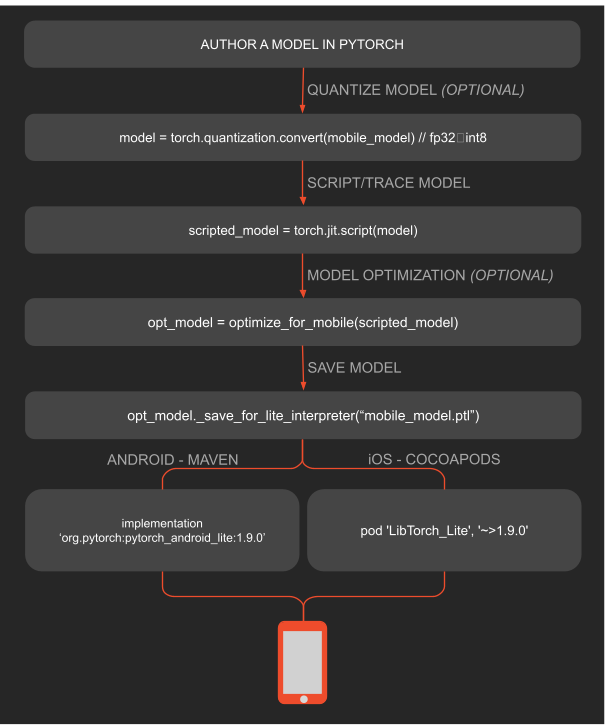
\includegraphics[scale = 0.6]{imagenes/pytorch-mobile.png}
	\caption{Optimización de modelos con Pytorch Mobile \cite{pmobile}}
	\label {fig:mobileprocess}
\end{figure}

Su compatibilidad engloba Android y iOS, siendo este último sistema soportado oficialmente tras el comienzo de la realización de este TFG. Aun así, este proyecto fue concebido inicialmente para ser probado en dispositivos Android, ya que el hardware de estos dispositivos tiene un mayor rendimiento en CPU y GPU, así como un mejor soporte de las librerías de aprendizaje. iOS, al tratarse de un SO cerrado a dispositivos Apple, y difícilmente emulable si no se dispone de dispositivos de la marca, requiere aún la existencia de frameworks estables dedicados al aprendizaje. Este motivo, sumando a que no disponemos de dispositivos con este sistema operativo, inclinó la balanza a usar únicamente dispositivos Android como dispositivo objetivo.

\subsection{Optimizaciones disponibles}

Pytorch mobile dispone para Android de una lista de 5 optimizaciones posibles a realizar sobre el modelo. Todas ellas, seleccionables de forma independiente, o aplicadas en conjunto por defecto, cubren los siguientes aspectos:

\begin{itemize}
	\item Fusión de las capa de convolución y normalización de batch: realiza una integración de los valores de normalización dentro de la capa convolutiva, ya que no será necesario reajustar esos valores para inferencia-
	\item Inserción y plegado de operaciones: utiliza la librería XNNPack, que se trata de un sistema de operaciones en coma flotante especialmente optimizado para ARM, que permite variar la precisión de los valores flotantes según el modelo. Fusiona las operaciones lineales y de convolución, de forma que se realicen en un menor tiempo.
	\item Fusión de la función ReLu con el conjunto de operaciones empaquetado creado con XNNPack en el paso anterior.
	\item Eliminación del dropout, ya que en tiempo de inferencia, se busca el mejor resultado si necesidad de reentreno.
	\item Optimización del grafo interno del modelo correspondiente a la convolución, para hacer que formen parte de un solo bloque raiz y mejore el tiempo de inferencia.	
\end{itemize}

En total, la web  \cite{pmobile} estima una ganancia aproximada del 60\% en tiempo de inferencia de forma teórica. Sin embargo, este valor puede oscilar en función de los datos que se estén evaluando, la arquitectura que deseamos cuantizar, y las capacidades de cálculo del dispositivo objetivo. A continuación, estudiaremos los resultados ofrecidos, y si merece la pena la aplicación de este proceso.

\section{Creación de los modelos cuantizados}

La transformación de los modelos entrenados a su versión cuantizada puede realizarse de forma inmediata, ya que en los pasos anteriores, el modelo entrenado sobre cada uno de los casos (clasificación binaria, y multiclase para benigno y maligno) fue almacenado en un fichero de formato .pt (extensión de modelo Pytorch).

Al tratarse de una conversión post-entrenamiento, no se requiere ningún ajuste de parámetros previo durante el entrenamiento, lo cual significa el entrenamiento sobre los modelos preparados para cuantización (QAT, o Quantization Aware Training  \cite{kuzmin2024fp8}), con el coste de una pequeña pérdida respecto a dicha ténica.

Para cuantizar el modelo tras su entrenamiento, basta con realizar los siguientes pasos:
\begin{enumerate}
	\item Cargar el modelo entrenado previamente. Como en nuestro caso, hemos realizado el salvado del modelo y procedemos a realizar la cuantización en el mismo en el mismo script, podemos directamente emplear el objeto Learner que almacena el modelo completo. En caso de que se quisiese leer de disco duro, bastaría con usar la función model.load().
	\item Activar el modo de evaluación del modelo. De esta forma, bloqueamos los parámetros libres de las capas de normalización de batches, y la aplicación de dropout.
	\item En este punto, podemos optar por dos opciones:
	\begin{enumerate}
		\item Exportar el modelo a Android sin ninguna optimización estructural, más allá de la adaptación de tipos de flotantes (función \textit{save\_for\_lite\_interpreter})
		\item Exportar el modelo aplicando todas las optimizaciones anteriores mencionadas para obtener el modelo más eficiente posible (función \textit{export\_for\_mobile})
	\end{enumerate}
	\item (Opcional) : exportar el modelo de escritorio en formato torch script. Se trata de un lenguaje de representación universal del modelo, que puede ser empleado con python nativo, y ser transferido a otros frameworks de trabajo habituales.
		
\end{enumerate}

Para realizar la comparativa de forma lo más exhaustiva posible, tomaremos el modelo de Android, y lo evaluaremos con el conjunto completo de imágenes de test, de forma que la valoración obtenida sea completamente representativa.

El pseucódigo resultante es batante sencillo, y su explicación queda prácticamente autocontenida gracias al uso de nombres de función represetativos:

\begin{algorithm}[H]
	\label{fig:cuantizado}
	\caption{Proceso de cuantizado de modelos a Android}
	\begin{algorithmic}
		\Procedure{exportar\_modelo}{learner: Learner Model Object, savename : String}
	
		\State model = learner.model.to('cpu') : Model
		\ State model.eval()
		
		 \State scripted\_module = torch.jit.script(nn.Sequential(model, Softmax(dim=n))) \\
		\Comment{Exportación del modelo original}
	 	 \State scripted\_module.save(savename + ``Full.pt")\\  
		 \Comment{Exportación del modelo optimizado}
		 \State optimized\_scripted\_module = optimize\_for\_mobile(scripted\_module) 
		 \State optimized\_scripted\_module.\_save\_for\_lite\_interpreter(savenameFull+ ``\_androidOptimized.pt")
	
		\EndProcedure
		
	\end{algorithmic}
\end{algorithm}

Podemos observar que el proceso es trivial, a excepción del último punto, donde se realiza la definición de un objeto de tipo sencuencial. Esto se debe que, cuando exportamos el modelo a Android, existen dos posibles alternativas para interpretar la capa de salida del mismo:
\begin{enumerate}
	\item Interpretando el tensor de salida de la función Softmax por columnas, de forma que la clase predicha para cada imagen será el máximo valor softmax encontrado en la columna en cuestión. En Python, se le conoce como máximo en dimensión 0, al tratarse del máximo de todas las filas.
	\item Interprentando el tensor de salida por filas, donde una imagen de entrenada recibe como etiqueta de salida el índice de la posición de fila cuyo valor es mayor. En este caso, se considera como dimensión 1, ya que se trata del valor máximo encontrado entre las columnas.
 \end{enumerate}

Por tanto, antes de exportar el modelo, será necesario especificar la dimensión de lectura. En versiones anteriores, esta dimensión era elegida de forma implícita por la función, pero ahora, debemos especificarla explícitamente para tener un correcto funcionamiento. Como en nuestro caso, solo tenemos una dimensión de etiquetas por modelos, debemos seleccionar el valor máximo por columnas, y valor a especificar es dim=1. Basta con crear un objeto de tipo Softmax, y especificar como parámetro \textit{dim}, el valor dim = 1.

Para concatenar el modelo original, y la nueva capa específica para la función Softmax, es necesario añadir ambos pasos a un pipeline, usando para la clase Sequential de Pytorch, que no es más que la creación de un modelo por capas.\\

Por último, para el proceso de comparación de modelos, realizaremos dos tareas:
\begin{enumerate}
	\item Evaluación del conjunto de test. Se realiza la inferncia completa del conjunto de test para estudiar la pérdida de rendimiento del modelo cuantizado frente al original haciendo uso un estimador insesgado, debido a la reserva de las imágenes hasta este momento.
	\item Comparativa de tiempos de inferencia. Realizaremos una comparativa de ejecución de ambos modelos en Android para evaluar la ganancia en tiempo tras aplicar cuantización, y si esta compensa las pérdidas de prestaciones. Debido a las limitaciones de la arquitectura ARM, evaluaremos el tiempo sobre una muestra del total, debido a la generación de calor y el desgaste ocasionado por la evaluación del test, que al tratarse del 40\% del cómputo global de imágenes, incluye 21478 fotografías.

\end{enumerate}

\section{Comparativa de los modelos original y cuantizado}

En este apartado, una vez comprendido el proceso de exportación y cuantización, examinaremos el rendimiento de cada uno de los 3 modelos creados para el proyecto. Para ello, evaluaremos el conjunto de test, intacto hasta esta fase, para conocer el rendimiento real de los modelos originales, y los compararemos con cada uno de los modelos cuantizados.

\subsection{Cuantización del modelo binario}

El modelo de clasificación binaria, que decide si la enfermedad se trata de un caso benigno o maligno, es la capa más importante de la arquitectura de dos niveles implementada. Su rendimiento es crítico dentro del funcionamiento del modelo, debido a que la confusión entre subtipos de enfermedades tiene un coste relativamente pequeño, pero un error entre una enfermedad cancerígena o benigna tiene un elevado coste para el paciente en consecuencias. Por tanto, es clave evaluar el modelo con el conjunto de test para conocer la bonanza del mismo, y estudiar si las gancias en espacio y tiempo de inferencia justifican la cuantización.\\

Evaluaremos el conjunto de test bajo las mismas condiciones, sin ningún tipo de preprocesado, más allá de la normalización de las imágenes y el reescalado a 512 x 512. Es muy importante destacar que estos valores son los mismos que los empleados en la fase de entrenamiento, ya que recalcular la media y desviación típica podría crear mejores resultados pero no ser una prueba representativa, ya que al realizar una inferencia de un diagnóstico, esta normalmente se realiza con una única imagen, y no habría datos suficientes para hallar la media y desviación típica. Debemos trabajar siempre con los parámetros de entrenamiento para que la distribución sea la misma, verificando así las condiciones ya vista acerca de disponer de un estimador no sesgado con test.

A continuación, comparamos la inferencia de ambos modelos y la ganancia en tiempo de inferencia entre ellos.

\subsubsection{Métricas de inferencia en test}

En primer lugar, comenzamos por evaluar la pérdida de rendimiento del modelo cuantizado. Para ello, ejecutamos el proceso de inferencia con ambos modelos, y obtenemos la tabla de resultados para ambos.
Los resultados de ambos modelos, original y cuantizado, podemos apreciarlos en las tablas \ref{tab:bintestorig} y \ref{tab:bintestquant} respectivamente.

\begin{table}[!ht]
	\centering
	\begin{tabular}{|c|c|c|c|c|}
		\hline
		~ & Precision & Recall & F1-score & Support \\ \hline
		Benign & 0.90 & 0.89 & 0.89 & 16010 \\ 
		Malignant & 0.68 & 0.70 & 0.69 & 5468 \\ \hline
		~ & ~ & accuracy & 0.84 & 21478 \\ \hline
		Macro avg & 0.79 & 0.80 & 0.79 & 21478 \\ 
		Weighted avg & 0.84 & 0.84 & 0.84 & 21478 \\ \hline
	\end{tabular}
	\caption{Resultados de inferencia en test para el modelo original}
	\label{tab:bintestorig}
\end{table}



\begin{table}[!ht]
	\centering
	\begin{tabular}{|c|c|c|c|c|}
		\hline
		~ & Precision & Recall & F1-score & Support \\ \hline
		Benign & 0.90 & 0.89 & 0.89 & 16010 \\ 
		Malignant & 0.68 & 0.70 & 0.69 & 5468 \\ \hline
		~ & ~ & accuracy & 0.84 & 21478 \\ \hline
		Macro avg & 0.79 & 0.79 & 0.79 & 21478 \\ 
		Weighted avg & 0.84 & 0.84 & 0.84 & 21478 \\ \hline
	\end{tabular}
	\caption{Resultados de inferencia en test para el modelo cuantizado}
	\label{tab:bintestquant}
\end{table}

Podemos apreciar que el resultado obtenido en el modelo original es muy similar a los obtenidos con la partición de validación, por lo que el modelo ha funcionado correctamente con datos los cuales no ha visto hasta el momento. Concretamente, en media, el modelo original en validación nos ofrecía el mismo resultado:  0.79 de precisión, 0.79 de recall,  0.79  de F1 Score y 0.84 de accuracy (\ref{tab:resultsbinrn50}). Si comparamos en detalle, hemos perdido recall y precisión en la clase maligna a favor de un ligero aumento de dichas métricas en la clase benigna, arrojando el mismo resultado medio. 

Si ahora estudiamos el caso optimizado y cuantizado para Android, observamos que sorprendentemente, no se han perdido prestaciones: las métricas son prácticamente idénticas a las obtenidas en el modelo original sin optimizar, a diferencia del recall medio, una centésima menor, lo cual es posible que se deba a algún ejemplo cuya valoración se ha visto erróneamente clasificada, pero cuyo impacto global ha sido. Podríamos afirmar que para este modelo, el impacto de optimización no ha afectado al rendimiento del modelo, el cual ha conservado las mismas prestaciones, ya que la diferencia en recall es prácticamente despreciable.

Esto ha sido posible gracias a las capacidades del framework desarrollado por Pytorch, las cuales han funcionado adecuadamente, al haber elegido un modelo totalmente compatible con el proceso de cuantización y optimización \cite{comptquant}.\\

En conclusión, para el modelo de clasificación binaria, obtenemos un modelo optimizado sin pérdida de rendimiento.

\subsubsection{Tiempo de inferencia}

Tras obtener unos buenos resultados en las métricas del modelo, podemos evaluar el tiempo medio de inferencia del modelo cuantizado frente al original en Android. Este factor es clave, ya que si el modelo cuantizado no ofrece resultados más eficientes en tiempo, el proceso de cuantizado no supone ninguna ventaja sobre el modelo original, sobre todo en este modelo, el cual ha demostrado no perder prestaciones en cuanto a métricas.

Los resultados se han tomado teniendo en cuenta únicamente la inferencia de 200 imágenes, debido a que la evaluación de las 21478 imágenes en un dispositivo móvil produce un sobrecalentamiento y desgaste considerable sobre los componentes. El terminal empleado hace uso de un Snapdragon 855, y 8GB de RAM, siendo estos componentes del año 2019, y arroja los siguientes resultados:

\begin{table}[H]
	\centering
	\begin{tabular}{|c|c|c|}
		\hline
		Modelo & Tiempo total (ms) & Tiempo medio (ms) \\ \hline
		Original & 114342 & 571,71 \\ \hline
		Cuantizado & 72352 & 361,76 \\ \hline
	\end{tabular}
	\caption{Tiempos de inferencia para caso binario en Android}
	\label{infbin}
\end{table}

Tras la evaluación del modelo mediante 200 imágenes, podemos apreciar una ganancia significativa en tiempo, superior a 210ms por imagen. Si calculamos la ganancia en velocidad del modelo cuantizado sobre el original, obtenemos:

$$Ganancia = \frac{t\ original}{t\ cuantizado} = \frac{571,71}{361,76} = 1.58$$

Es decir, el modelo optimizado nos aporta uan ganancia de 1.58, lo cual supone aproximadamente un 40\% menos del tiempo de inferencia. Este resultado evidencia que el modelo cuantizado ofrece unas mejores prestaciones que el original. Teniendo en cuenta que el modelo cuantizado no pierde bondad de métricas al ser evaluado con el conjunto de test frente al original, queda demostrado que el modelo cuantizado supone una mejora considerable y debe ser el modelo a utilizar en un dispositivo móvil. La penalización obtenida es nula, y las ventajas, cuantiosas.

\subsection{Cuantización del modelo maligno}

El modelo de clasificación de enfermedades malignas se del primero de los casos de clasificación multiclase. A diferencia del anterior, este modelo aporta una salida más compleja, al deber distinguir entre melanomas, cáncer de células basales y cáncer de células escamosas. Esto nos deja un con vector de salida de 3 componentes, una por cada clase, que el modelo deberá aportar tanto en el modelo original como el cuantizado.

De la misma manera que con el caso de clasificación binaria, compararemos los dos modelos mediante la evaluación del conjunto de test, teniendo en cuenta que las imágenes ha de ser preprocesadas con los mismos parámetros y configuraciones del conjunto de test, y no recalcular ninguno de los valores. Este preprocesado, al igual que en entrenamiento, incluye:

\begin{enumerate}
	\item Renombrado de etiquetas. Al igual que en el modelo de entrenamiento decidimos fusionar las clases melanoma y melanoma metastasis, debemos de aplicar la misma transformación en test. Si no lo hiciésemos, el modelo funcionaría adecuadamente, pero no podríamos evaluar correctamente las métricas que nos permiten ver si el rendimiento es el esperado.
	 \item Normalización y resize: se utilizan la media y desviación típica de imagenet, empleadas en entrenamiento, y se aplica un resize de 512 x 512 px siguiendo la misma distribución.
\end{enumerate}

Una vez realizado este preprocesado, podemos calcular la inferencia de los dos modelos.

\subsubsection{Métricas de inferencia en test}
Para evaluar la calidad del modelo cuantizado, se tomarán tanto el modelo original como el cuantizado, ambos exportados durante el aprendizaje realizado en el capitulo 5, y obtendremos la tabla resumen de métricas para realizar la comparativa.
Los resultados  podemos apreciarlos en las tablas \ref{tab:maltestorig} (original) y \ref{tab:maltestquant}(cuantizado).

\begin{table}[!ht]
	\centering
	\begin{tabular}{|c|c|c|c|c|}
		\hline
		~ & Precision & Recall & F1-score & Support \\ \hline
		Basal Cell C. & 0.80 & 0.84 & 0.82 & 1969 \\
		Melanoma & 0.87 & 0.92 & 0.89 & 2950 \\
		Squamous Cell C. & 0.65 & 0.37 & 0.47 & 549 \\ \hline
		Accuracy & ~ & ~ & 0.83 & 5468 \\ \hline
		Macro avg & 0.78 & 0.71 & 0.73 & 5468 \\
		Weighted avg & 0.83 & 0.83 & 0.83 & 5468 \\ \hline
	\end{tabular}
	\caption{Resultados de inferencia en test para el modelo original}
	\label{tab:maltestorig}
\end{table}

\begin{table}[!ht]
	\centering
	\begin{tabular}{|c|c|c|c|c|}
		\hline
		~ & Precision & Recall & F1-score & Support \\ \hline
		Basal Cell C. & 0.80 & 0.84 & 0.82 & 1969 \\
		Melanoma & 0.87 & 0.92 & 0.89 & 2950 \\
		Squamous Cell C. & 0.65 & 0.37 & 0.47 & 549 \\ \hline
		Accuracy & ~ & ~ & 0.83 & 5468 \\ \hline
		Macro avg & 0.78 & 0.71 & 0.73 & 5468 \\
		Weighted avg & 0.83 & 0.83 & 0.83 & 5468 \\ \hline
	\end{tabular}
	\caption{Resultados de inferencia en test para el modelo cuantizado}
	\label{tab:maltestquant}
\end{table}

En este subproblema, encontramos que ambos modelos arrojan exactamente el mismo resultado, por lo que el proceso de optimización no ha conllevado ninguna pérdida para el rendimiento del modelo, lo cual es un caso totalmente ideal. Para ver su rendimiento real, podemos comparar el modelo con el resultado arrojado por el conjunto de validación:  0.79 de precisión,  0.72 de recall, y  0.74 de F1 Score (tabla \ref{tab:malignometrics}).  Podemos apreciar que, por tanto, el conjunto de validación fue un correcto estimador de las funciones de pérdida y métricas fuera de la muestra.

Por tanto, el modelo cuantizado, y a su vez, el original, ofrecen un muy buen resultado, acorde a lo estimado durante el entrenamiento, y sin pérdida de precisión de clasificación en el caso del modelo cuantizado. 

\subsubsection{Tiempo de inferencia}

Tras observar que el modelo cuantizado no supone pérdidas sobre el modelo original, un caso ideal, nos disponemos a evaluar el tiempo de inferencia por imagen, de la misma manera que se realizó con el modelo binario.

Se usará el mismo dispositivo, empleando un subconjunto para la inferencia de 200 imágenes. Los resultados se pueden apreciar en la siguiente tabla:

\begin{table}[H]
	\centering
	\begin{tabular}{|c|c|c|}
		\hline
		Modelo & Tiempo total (ms) & Tiempo medio (ms) \\ \hline
		Original & 215693 & 1078,465	 \\ \hline
		Cuantizado & 136912 & 684,56 \\ \hline
	\end{tabular}
	\caption{Tiempos de inferencia para caso binario en Android}
	\label{infbin}
\end{table}

A la vista de los resultados, podemos apreciar una ganancia significativa en tiempo, de alrededor de 394ms por imagen. A priori, parece que el ahorro en tiempo es mayor que en el caso binario, pero si calculamos la ganancia en velocidad, obtenemos:

$$Ganancia = \frac{t\ original}{t\ cuantizado} = \frac{1078,465}{684,56} = 1.575$$

Es decir, el modelo optimizado nos aporta una ganancia de 1.575, lo cual es proporción es prácticamente la misma ganancia que la conseguida con la cuantización en caso binario. De nuevo, supone aproximadamente un 37\% menos de tiempo de inferencia sobre el modelo original. 
En conclusión, el modelo a utilizar como modelo final vuelve a ser la versión cuantizada, ya que nos permite mejorar considerablemente el rendimiento sin pérdida de prestaciones.